%! Tex program = pdflatex
 
\documentclass[UTF8]{ctexart}
\CTEXsetup[format={\Large\bfseries}]{section}
\usepackage{amsmath}
\usepackage{ctex}
\usepackage{array}
\usepackage{ulem}
\usepackage{graphicx}
\usepackage{geometry}
\usepackage{multirow}
\usepackage{subfig}
\usepackage{float}
\usepackage{multicol}
\usepackage{multirow}
\usepackage{indentfirst}
\usepackage{makecell}
\usepackage{listings, xcolor}
\lstdefinestyle{lfonts}{
  basicstyle   = \footnotesize\ttfamily,
  stringstyle  = \color{purple},
  keywordstyle = \color{blue!60!black}\bfseries,
  commentstyle = \color{olive}\scshape,
}
\lstdefinestyle{lnumbers}{
  numbers     = left,
  numberstyle = \tiny,
  numbersep   = 1em,
  firstnumber = 1,
  stepnumber  = 1,
}
\lstdefinestyle{llayout}{
  breaklines       = true,
  tabsize          = 2,
  columns          = flexible,
}
\lstdefinestyle{lgeometry}{
  xleftmargin      = 20pt,
  xrightmargin     = 0pt,
  frame            = tb,
  framesep         = \fboxsep,
  framexleftmargin = 20pt,
}
\lstdefinestyle{lgeneral}{
  style = lfonts,
  style = lnumbers,
  style = llayout,
  style = lgeometry,
}
\lstdefinestyle{python}{
  language = {Python},
  style    = lgeneral,
}
\geometry{papersize={21cm,29.7cm}}
\geometry{left=2.54cm,right=2.54cm,top=3.18cm,bottom=3.18cm}
\usepackage{fancyhdr}
\pagestyle{fancy}
\lhead{\today}
\chead{}
\rhead{2020011075}
\lfoot{清华大学}
\cfoot{\thepage}
\rfoot{系统工程导论}
\renewcommand{\headrulewidth}{0.4pt}
\renewcommand{\headwidth}{\textwidth}
\renewcommand{\footrulewidth}{0pt}
\usepackage{bm}

\begin{document}

\begin{center}
  \textbf{\LARGE{系统工程导论作业六——聚类分析}}\\
\end{center}
\begin{center}
  \large{彭程 2020011075}
\end{center}


\noindent \textbf{\zihao{-4}{1.K-means}}

\noindent \textbf{\zihao{-4}{1.1 自行编写 K-means 聚类算法,绘制 3 个数据集的聚类结果}}

根据三个聚类的形状,分别选择 K 值为 2, 3, 3,得到的聚类结果如下:

\begin{figure}[H]
  \centering
  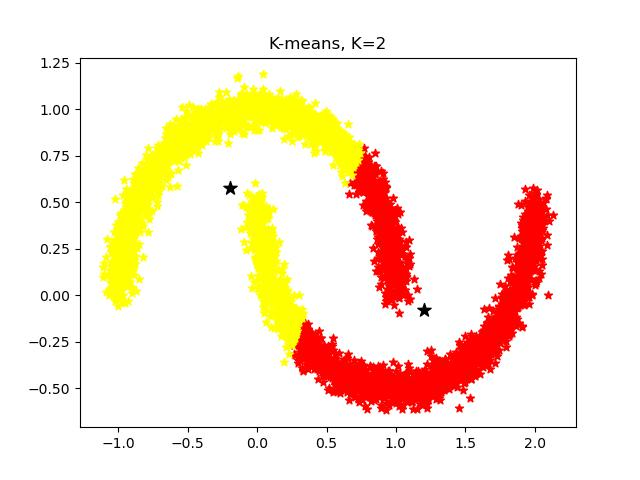
\includegraphics[scale=0.46]{no1.jpg}
\end{figure}

\begin{figure}[H]
  \centering
  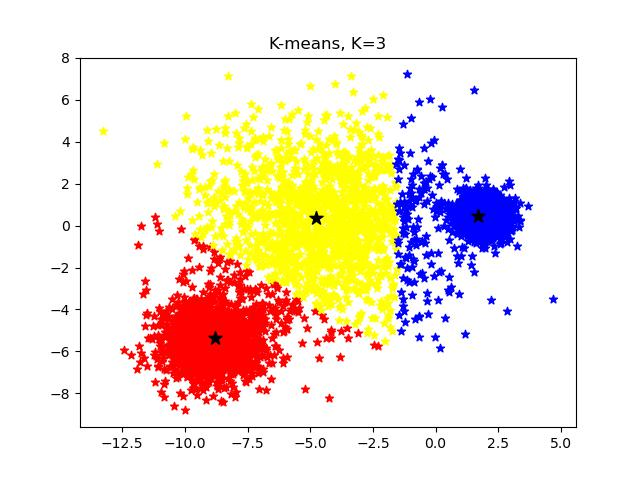
\includegraphics[scale=0.46]{no2.jpg}
\end{figure}

\begin{figure}[H]
  \centering
  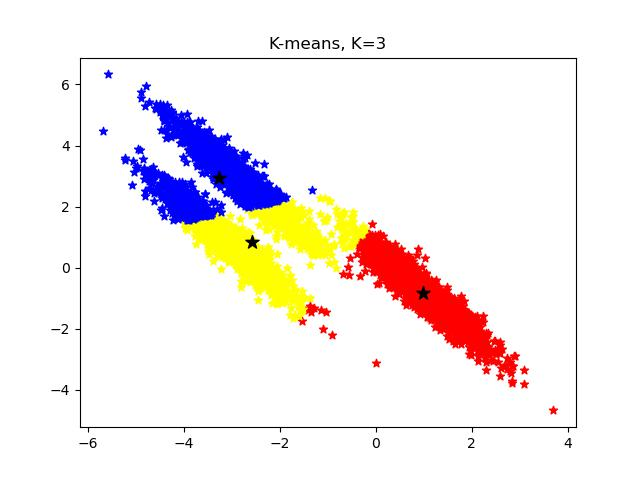
\includegraphics[scale=0.46]{no3.jpg}
\end{figure}

\noindent \textbf{\zihao{-4}{1.2.利用数据集 data2,对 K-means 算法进行如下实验}}

\noindent \textbf{1.2.1} 增加聚类数目,计算并分析聚类结果,决定最合适的聚类数目并说明理由

$k=1\sim9 $的聚类结果如下:

\begin{figure}[H]
	\centering
	\begin{minipage}{0.32\linewidth}
		\centering
		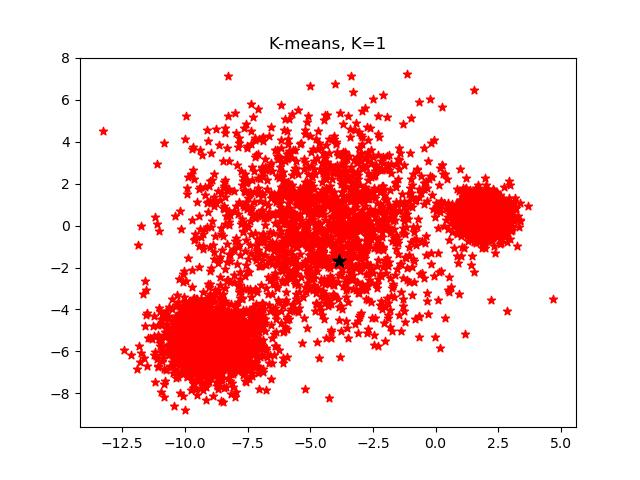
\includegraphics[width=0.9\linewidth]{k=1.jpg}
		\caption{k=1}
		\label{chutian1}%文中引用该图片代号
	\end{minipage}
	\begin{minipage}{0.32\linewidth}
		\centering
		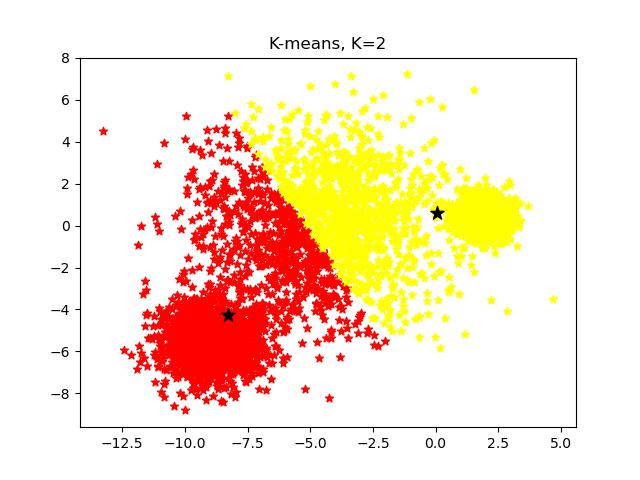
\includegraphics[width=0.9\linewidth]{k=2.jpg}
		\caption{k=2}
		\label{chutian2}%文中引用该图片代号
	\end{minipage}
  \begin{minipage}{0.32\linewidth}
		\centering
		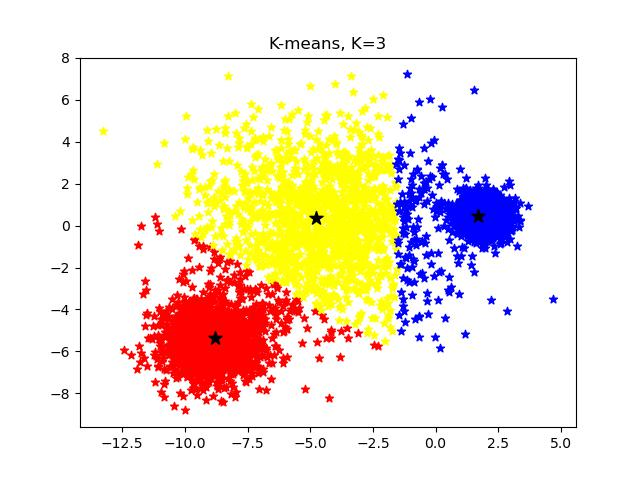
\includegraphics[width=0.9\linewidth]{k=3.jpg}
		\caption{k=3}
		\label{chutian2}%文中引用该图片代号
	\end{minipage}
	%\qquad
	%让图片换行,
  \begin{minipage}{0.32\linewidth}
		\centering
		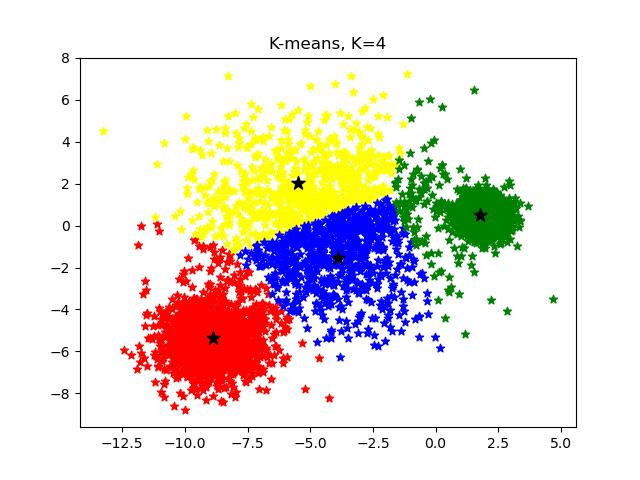
\includegraphics[width=0.9\linewidth]{k=4.jpg}
		\caption{k=4}
		\label{chutian1}%文中引用该图片代号
	\end{minipage}
	\begin{minipage}{0.32\linewidth}
		\centering
		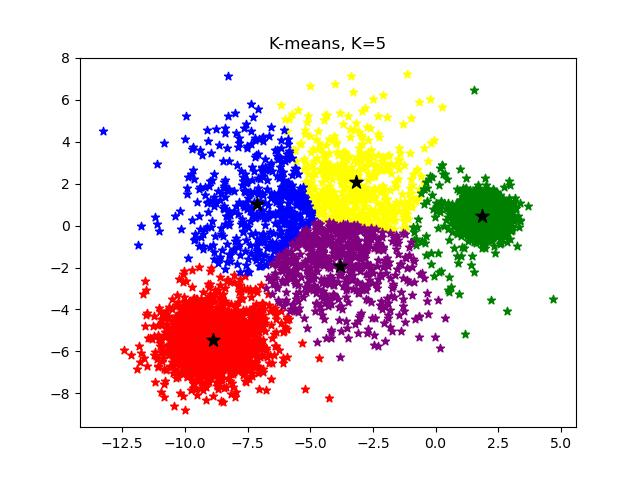
\includegraphics[width=0.9\linewidth]{k=5.jpg}
		\caption{k=5}
		\label{chutian2}%文中引用该图片代号
	\end{minipage}
  \begin{minipage}{0.32\linewidth}
		\centering
		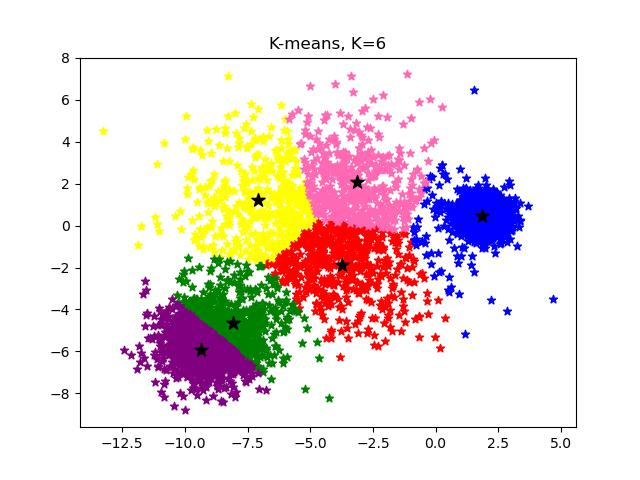
\includegraphics[width=0.9\linewidth]{k=6.jpg}
		\caption{k=6}
		\label{chutian2}%文中引用该图片代号
	\end{minipage}

  \begin{minipage}{0.32\linewidth}
		\centering
		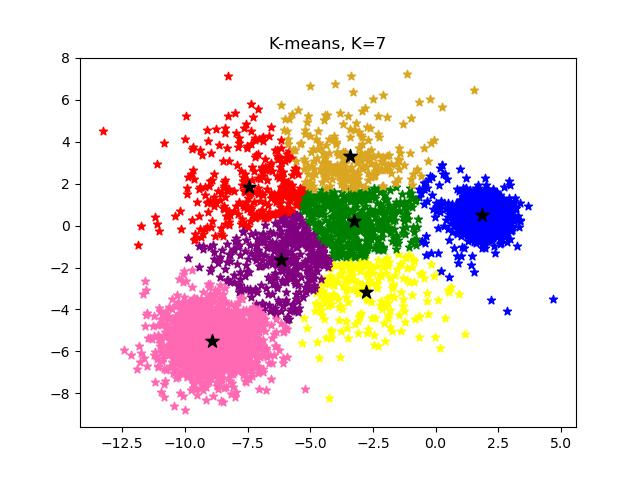
\includegraphics[width=0.9\linewidth]{k=7.jpg}
		\caption{k=7}
		\label{chutian1}%文中引用该图片代号
	\end{minipage}
	\begin{minipage}{0.32\linewidth}
		\centering
		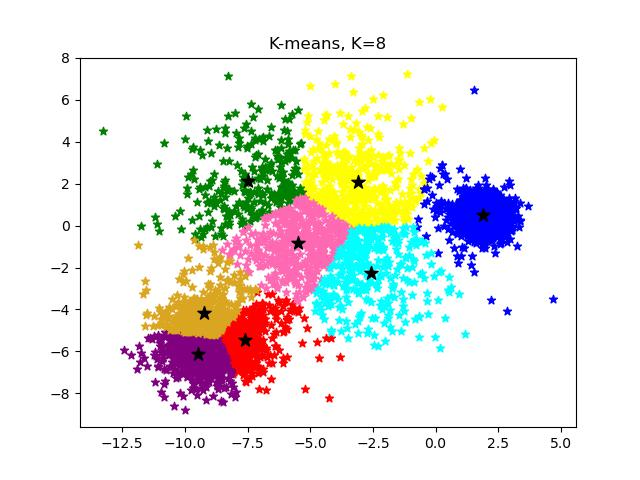
\includegraphics[width=0.9\linewidth]{k=8.jpg}
		\caption{k=8}
		\label{chutian2}%文中引用该图片代号
	\end{minipage}
  \begin{minipage}{0.32\linewidth}
		\centering
		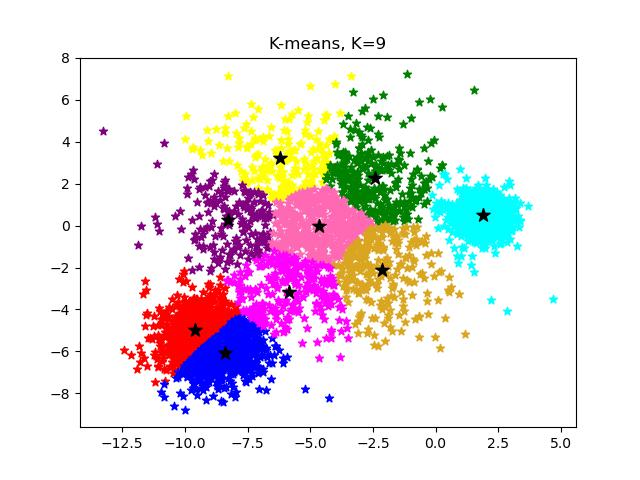
\includegraphics[width=0.9\linewidth]{k=9.jpg}
		\caption{k=9}
		\label{chutian2}%文中引用该图片代号
	\end{minipage}

\end{figure}

采用 elbow method 法则选取 $\mathrm{K}$, 即最小化点到聚类中心的距离之和:

$$
\sum_{i=0}^{n} \min _{\mu_{j} \in C}\left(\left\|x_{i}-\mu_{j}\right\|^{2}\right)
$$

绘制出的图像如下:

\begin{figure}[H]
  \centering
  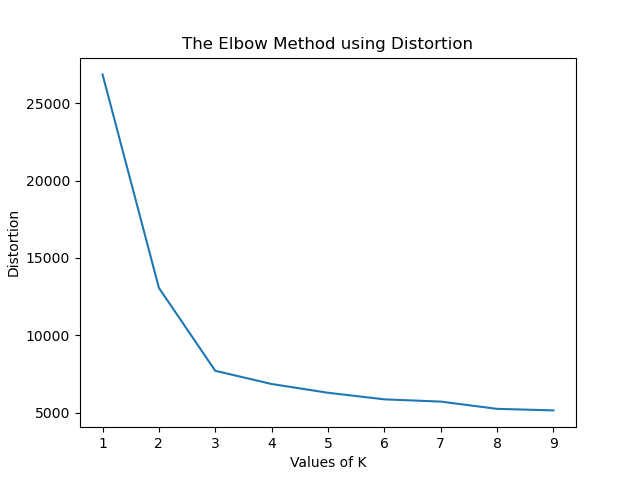
\includegraphics[scale=0.23]{myplot.png}
\end{figure}

故选择 k = 3。因为k>3后随k的增加,距离和的变换趋于平缓,增加k的代价过高。

\noindent \textbf{1.2.2} 选择不同的初始点多次实验,观察初始点的选择对最终结果的影响,并分析原因


\begin{figure}[H]
	\centering
  \begin{minipage}{0.32\linewidth}
		\centering
		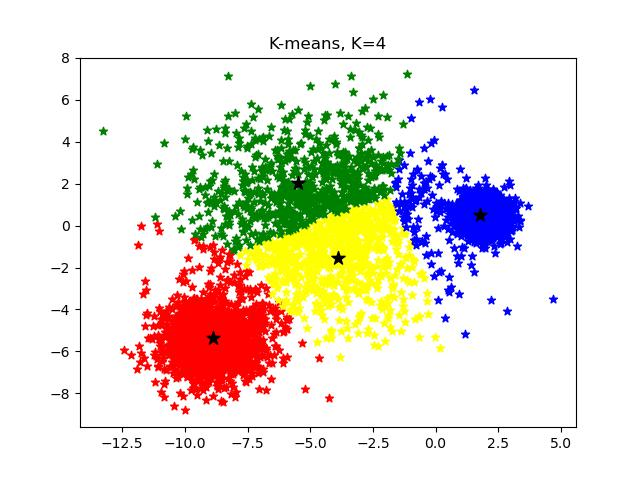
\includegraphics[width=0.9\linewidth]{no2-1.jpg}
	\end{minipage}
	\begin{minipage}{0.32\linewidth}
		\centering
		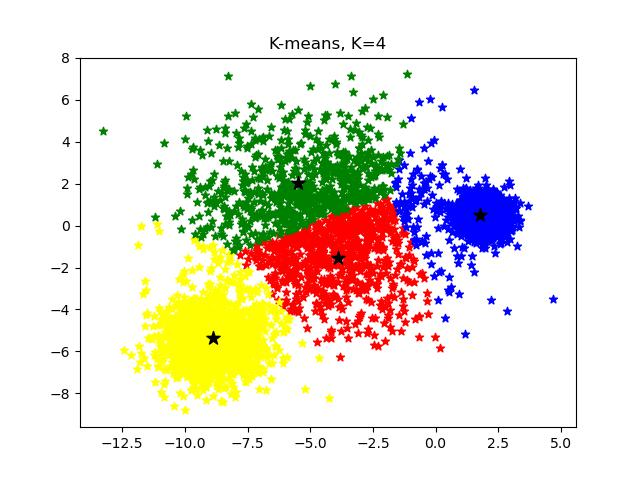
\includegraphics[width=0.9\linewidth]{no2-2.jpg}
	\end{minipage}
  \begin{minipage}{0.32\linewidth}
		\centering
		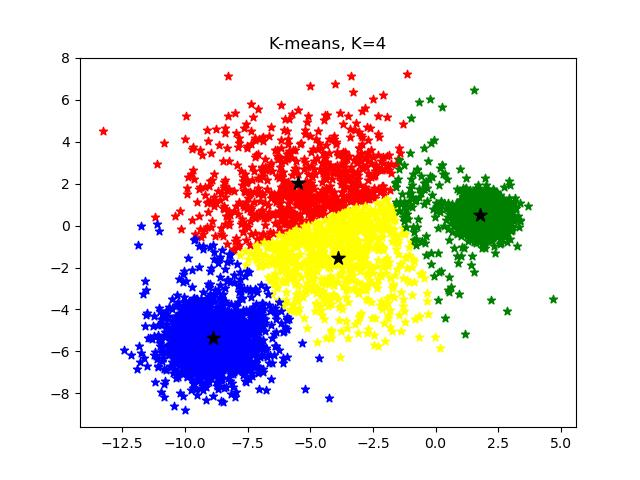
\includegraphics[width=0.9\linewidth]{no2-3.jpg}
	\end{minipage}

\end{figure}

选择不同的初始点进行多次实验,发现最终都收敛到了相同的中心点(如上),只是由于初始点不同,在收敛时间上有差异。

这可能是因为data2自身的点分布比较分散且均匀,于是我们对data1进行了实验,结果如下:


\begin{figure}[H]
	\centering
  \begin{minipage}{0.32\linewidth}
		\centering
		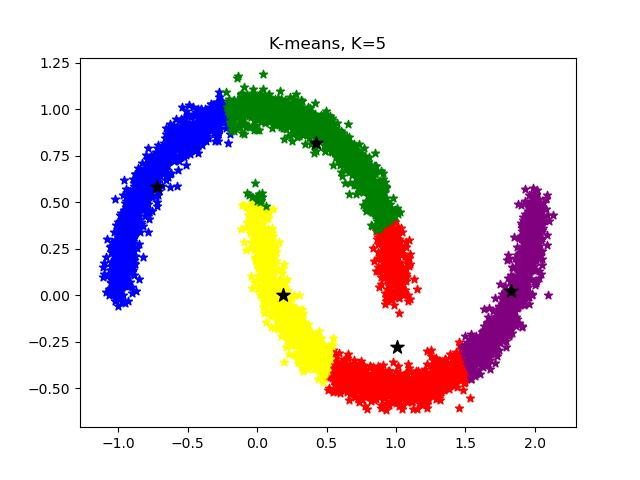
\includegraphics[width=0.9\linewidth]{no1-1.jpg}
	\end{minipage}
	\begin{minipage}{0.32\linewidth}
		\centering
		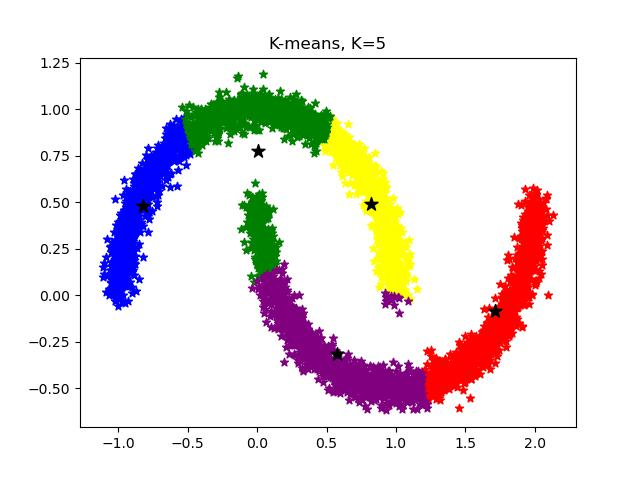
\includegraphics[width=0.9\linewidth]{no1-2.jpg}
	\end{minipage}
  \begin{minipage}{0.32\linewidth}
		\centering
		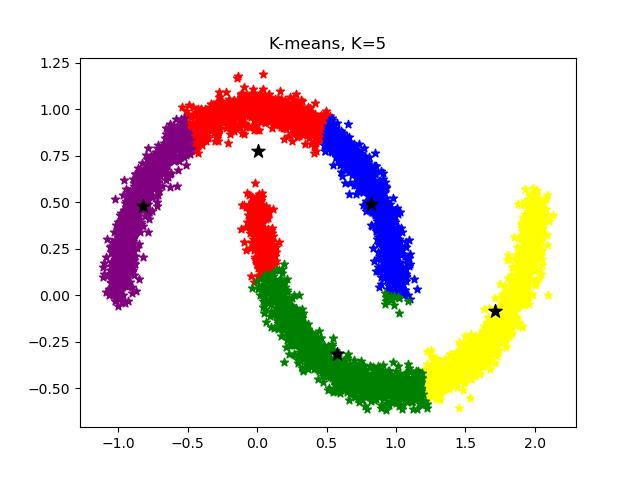
\includegraphics[width=0.9\linewidth]{no1-3.jpg}
	\end{minipage}

\end{figure}

对于data1的实验我们得到了不同的结果,这是因为 K-means 算法初始点选取不同时,虽然能保证收敛到某一个结果,但不能保证每次收敛到同一个结果,最后的结果可能是不稳定的,也可以理解为陷入局部的极值。\\

\noindent \textbf{\zihao{-4}{2.DBSCAN}}\\


\noindent \textbf{\zihao{-4}{2.1 自行编写 DBSCAN 聚类算法,绘制 3 个数据集的聚类结果}}

得到的聚类结果如下:

\begin{figure}[H]
  \centering
  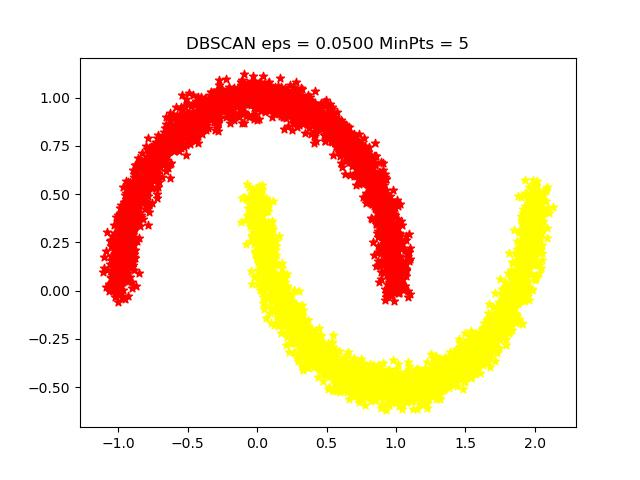
\includegraphics[scale=0.46]{data1.jpg}
\end{figure}

\begin{figure}[H]
  \centering
  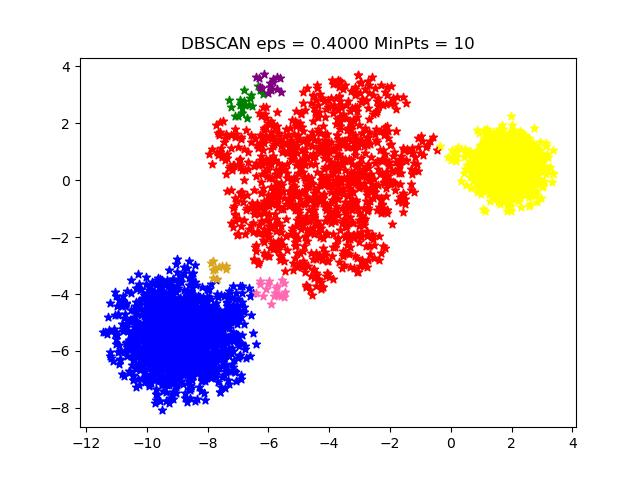
\includegraphics[scale=0.46]{data2.jpg}
\end{figure}

\begin{figure}[H]
  \centering
  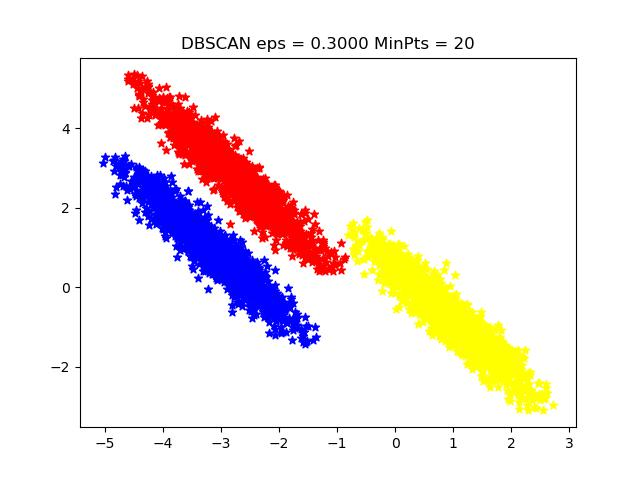
\includegraphics[scale=0.46]{data3.jpg}
\end{figure}

\noindent \textbf{\zihao{-4}{2.2 利用数据集 data3,对DBSCAN算法进行如下实验}}

\noindent \textbf{2.2.1}选择不同的$\epsilon$,观察实验结果并分析原因;

$\epsilon$分别取0.01,0.1,0.2,0.3,0.4,0.5的聚类结果如下所示:

\begin{figure}[H]
	\centering
	\begin{minipage}{0.32\linewidth}
		\centering
		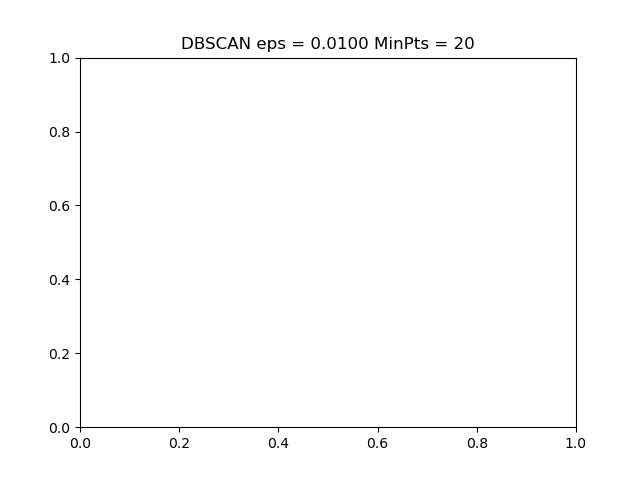
\includegraphics[width=0.9\linewidth]{data3-0.01.jpg}
		\caption{$\epsilon=0.01$}
		\label{chutian1}%文中引用该图片代号
	\end{minipage}
	\begin{minipage}{0.32\linewidth}
		\centering
		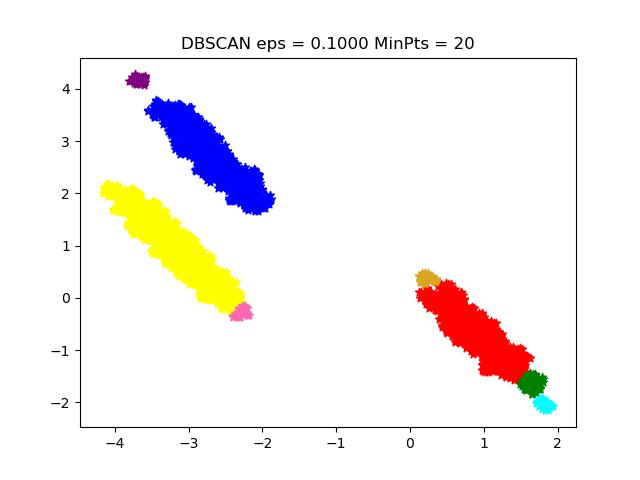
\includegraphics[width=0.9\linewidth]{data3-0.1.jpg}
		\caption{$\epsilon=0.1$}
		\label{chutian2}%文中引用该图片代号
	\end{minipage}
  \begin{minipage}{0.32\linewidth}
		\centering
		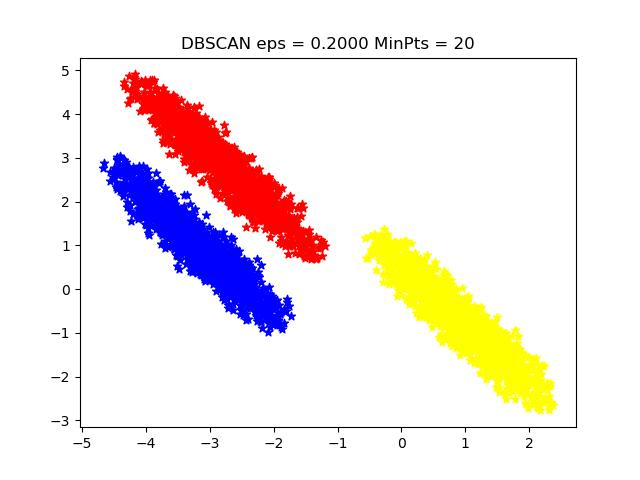
\includegraphics[width=0.9\linewidth]{data3-0.2.jpg}
		\caption{$\epsilon=0.2$}
		\label{chutian2}%文中引用该图片代号
	\end{minipage}
	%\qquad
	%让图片换行,
  \begin{minipage}{0.32\linewidth}
		\centering
		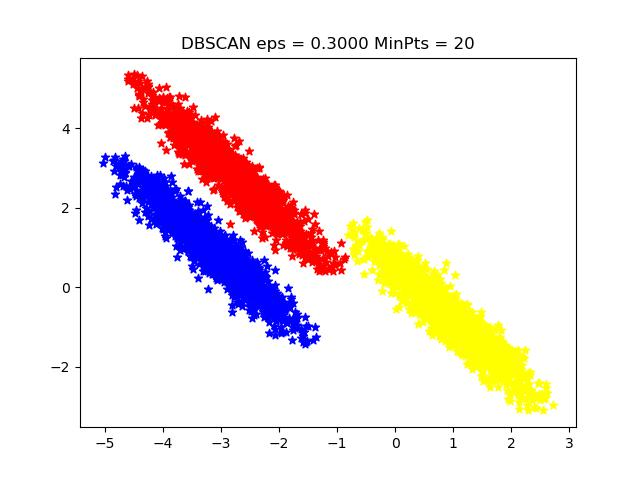
\includegraphics[width=0.9\linewidth]{data3-0.3.jpg}
		\caption{$\epsilon=0.3$}
		\label{chutian1}%文中引用该图片代号
	\end{minipage}
	\begin{minipage}{0.32\linewidth}
		\centering
		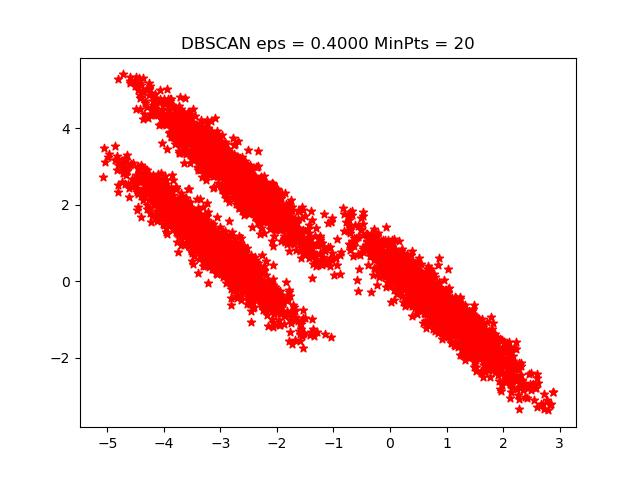
\includegraphics[width=0.9\linewidth]{data3-0.4.jpg}
		\caption{$\epsilon=0.4$}
		\label{chutian2}%文中引用该图片代号
	\end{minipage}
  \begin{minipage}{0.32\linewidth}
		\centering
		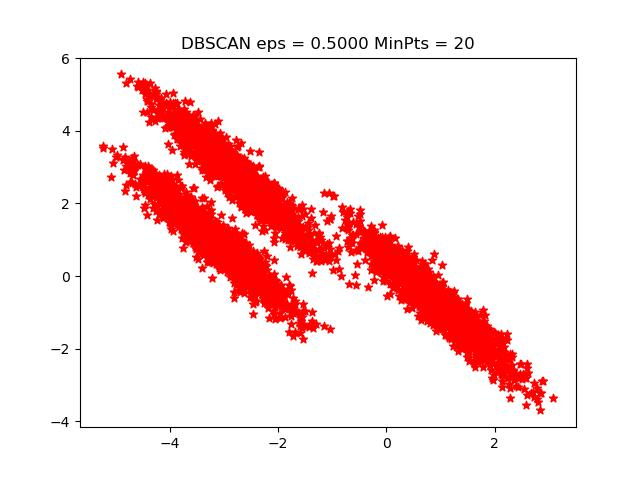
\includegraphics[width=0.9\linewidth]{data3-0.5.jpg}
		\caption{$\epsilon=0.5$}
		\label{chutian2}%文中引用该图片代号
	\end{minipage}
\end{figure}

$\epsilon=0.01$时半径选取过小,导致不存在核心点。
$\epsilon=0.1$时半径仍然较小,导致把同一类的样本点拆分成了几类。
$\epsilon=0.2,0.3$时半径合适,分类结果较为可靠。
$\epsilon=0.4,0.5$时半径过大,几个类会被粘连到一起,导致聚类效果变差。\\




\noindent \textbf{2.2.2}选择不同的$minPots$, 观察实验结果并分析原因; 



\begin{figure}[H]
	\centering
	\begin{minipage}{0.32\linewidth}
		\centering
		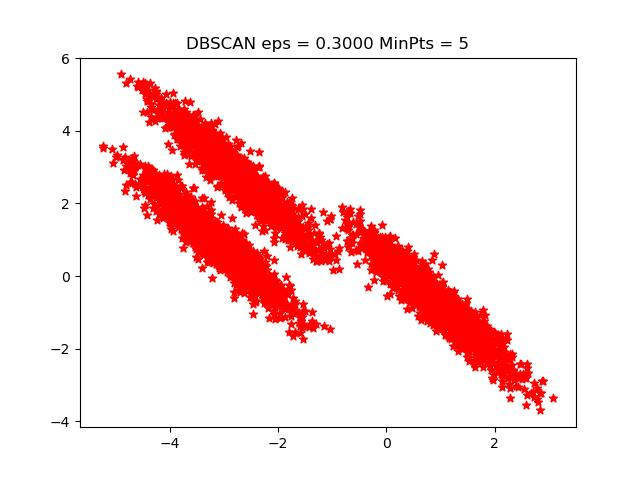
\includegraphics[width=0.9\linewidth]{data3-5.jpg}
		\caption{$minPots=5$}
		\label{chutian1}%文中引用该图片代号
	\end{minipage}
	\begin{minipage}{0.32\linewidth}
		\centering
		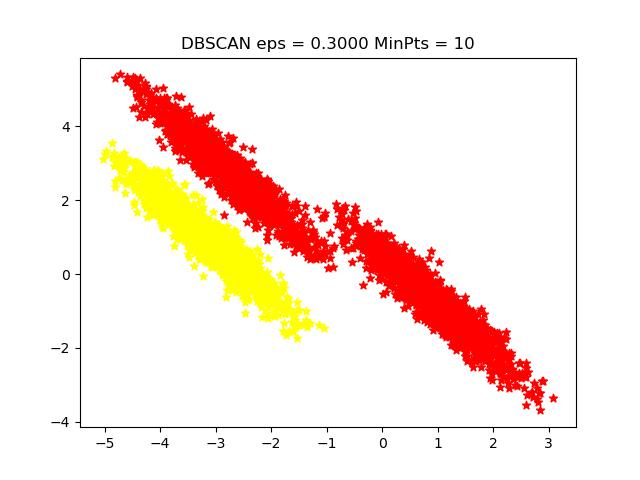
\includegraphics[width=0.9\linewidth]{data3-10.jpg}
		\caption{$minPots=10$}
		\label{chutian2}%文中引用该图片代号
	\end{minipage}
  \begin{minipage}{0.32\linewidth}
		\centering
		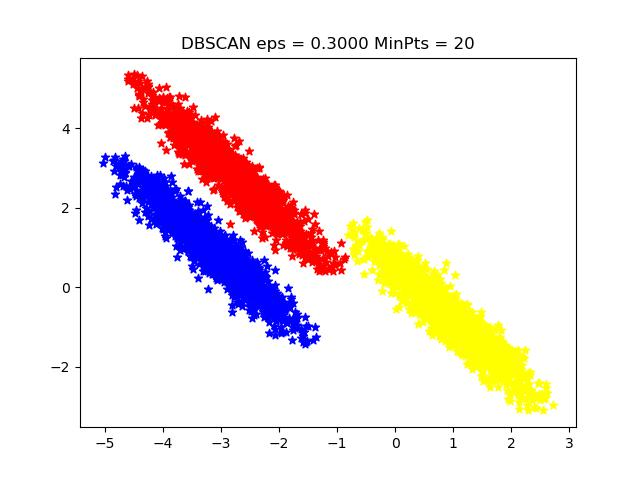
\includegraphics[width=0.9\linewidth]{data3-20.jpg}
		\caption{$minPots=20$}
		\label{chutian2}%文中引用该图片代号
	\end{minipage}
	%\qquad
	%让图片换行,
  \begin{minipage}{0.32\linewidth}
		\centering
		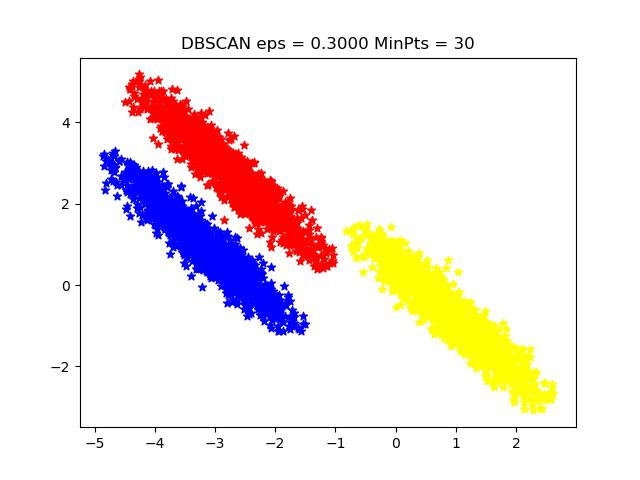
\includegraphics[width=0.9\linewidth]{data3-30.jpg}
		\caption{$minPots=30$}
		\label{chutian1}%文中引用该图片代号
	\end{minipage}
	\begin{minipage}{0.32\linewidth}
		\centering
		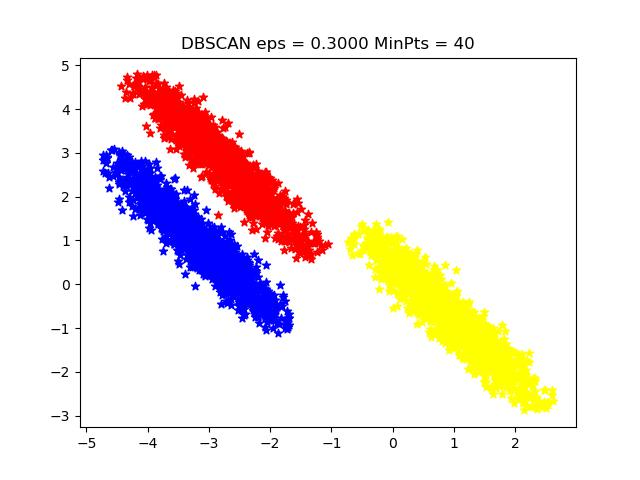
\includegraphics[width=0.9\linewidth]{data3-40.jpg}
		\caption{$minPots=40$}
		\label{chutian2}%文中引用该图片代号
	\end{minipage}
  \begin{minipage}{0.32\linewidth}
		\centering
		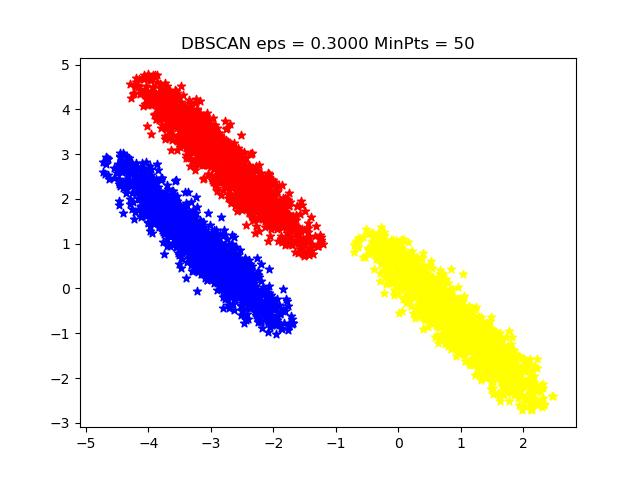
\includegraphics[width=0.9\linewidth]{data3-50.jpg}
		\caption{$minPots=50$}
		\label{chutian2}%文中引用该图片代号
	\end{minipage}
\end{figure}

当$\epsilon$一定时, 增大 MinPots 即意味着一个点要想成为核心点需要邻域内有更多的点,即使得一个点成为核心点的要求变高, 因而会导致部分原本的核心点被当作边界点或者被舍弃的噪声点,会把同一类的样本点拆分成几类,甚至导致不存在核心点;反之减小MinPots 会使得一个点成为核心点的要求变低, 因而会导致更多的边界点或者被舍弃的噪声
点会被当作核心点,甚至相距较近的几个类会被粘连到一起, 导致聚类效果变差。\\


\noindent \textbf{\zihao{-4}{3.对比分析kmeans和DBSCAN聚类算法}}

K-means 算法是基于划分的聚类算法, 算法简单、快速、易于实现, 比较适合球状分布的聚类, 而且不受点的密度的影响, 聚类的结果易于解释, 但是可能会陷入局部最优, 对离群点和噪声点敏感, 不同初始点的选取可能会导致不同的聚类结果。

DBSCAN 算法是基于密度的聚类算法, 可以对任意形状的稠密数据集进行聚类, 而且可以在聚类的同时发现噪音点, 不需要事先指定类别数目, 聚类结果也不依赖节点的遍历顺序, 但是数据集过大时,收敛时间长, 而且$\epsilon$、 MinPots选取较为困难。

具体到本次作业中的三组数据, 对于 data1 和 data3, DBSCAN 得到的聚类结果更好;
对于 data2, K-means 和 DBSCAN 效果相对来说比较接近,但 DBSCAN 的结果出现了许多
小聚类, K-means 则不会出现。 而且 K-means 收敛时间明显小于 DBSCAN 的收敛时间。

\end{document}